% !TeX TXS-program:compile = txs:///pdflatex/
% !TeX program = pdflatex
% !BIB program = biber


\section{Some Additional Figures}
\label{app:sec:AdditionalFigures}

\begin{figure}[h]
	\resizebox{\textwidth}{!}{%
		\begin{tikzpicture}
		
		
		\draw[->] (-9.5,0) -- (3.5,0); 
		\node at (-8.25,0.75) {$w$ weeks};
		\path[->] (-9,0.25) edge [bend left] (-7.5,0.25);
		\node at (0.75,0.75) {$w$ weeks};
		\path[->] (0,0.25) edge [bend left] (1.5,0.25);
		\node at (3.8,0) {$t$};
		%\node at (-10,0.2) {(i):}; % 1
		
		\draw (-9,0.075) -- (-9,-0.075); %node at (-9,0.3) {$1$};
		\draw (-7.5,0.075) -- (-7.5,-0.075); %node at (-7.5,0.3) {$2$};
		\draw (-6,0.075) -- (-6,-0.075); %node at (-6,0.3) {$3$};
		\draw (-4.5,0.075) -- (-4.5,-0.075); %node at (-4.5,0.3) {$4$};
		\draw (-3,0.075) -- (-3,-0.075); %node at (-3,0.3) {$5$};
		\draw (-1.5,0.075) -- (-1.5,-0.075); %node at (-1.5,0.3) {$6$};
		\draw (0,0.075) -- (0,-0.075); %node at (0,0.3) {$7$};
		\draw (1.5,0.075) -- (1.5,-0.075); %node at (1.5,0.3) {$8$};
		\draw (3,0.075) -- (3,-0.075); %node at (3,0.3) {$9$};
		
		
		\node at (-10.5,-.775) {$\cbalCL(1)$:};  % { A$_{\text{conc},b,r,w}$=1:}; 
		
		\node at (-9,-.75) {$1$};
		\node[align = center] at (-9,-1.25) {$+$ \\ $B$};
		\node at (-7.5,-.75) {$1$};
		\node at (-6,-.75) {$1$};
		\node at (-4.5,-.75) {$1$};
		\node at (-3,-.75) {$1$};
		\node at (-1.5,-.75) {$1$};
		\node at (0,-.75) {$1$};
		\node at (1.5,-.75) {$1$};
		\node at (3,-.75) {$1$};
		
		\node at (-10.5,-2.275) {$\cbalCL(2)$:};
		\node at (-9,-2.25) {$1$};
		\node[align = center] at (-7.5,-2.75) {$+$ \\ $B + i$};
		\node at (-7.5,-2.25) {$1$};
		\node at (-6,-2.25) {$1$};
		\node at (-4.5,-2.25) {$1$};
		\node at (-3,-2.25) {$1$};
		\node at (-1.5,-2.25) {$1$};
		\node at (0,-2.25) {$1$};
		\node at (1.5,-2.25) {$1$};
		\node at (3,-2.25) {$1$};
		
		\node at (-10.5,-3.775) {$\cbalCL(3)$:}; 
		\node[align = center] at (-6,-4.25) {$+$ \\ $B + 2i$};
		\node at (-9,-3.75) {$1$};
		\node at (-7.5,-3.75) {$1$};
		\node at (-6,-3.75) {$1$};
		\node at (-4.5,-3.75) {$1$};
		\node at (-3,-3.75) {$1$};
		\node at (-1.5,-3.75) {$1$};
		\node at (0,-3.75) {$1$};
		\node at (1.5,-3.75) {$1$};
		\node at (3,-3.75) {$1$};
		
		\node at (-10.5,-5.275) {$\cbalCL(4)$:}; 
		\node[align = center] at (-4.5,-5.75) {$+$ \\ $B + 3i$};
		\node at (-9,-5.25) {$1$};
		\node at (-7.5,-5.25) {$1$};
		\node at (-6,-5.25) {$1$};
		\node at (-4.5,-5.25) {$1$};
		\node at (-3,-5.25) {$1$};
		\node at (-1.5,-5.25) {$1$};
		\node at (0,-5.25) {$1$};
		\node at (1.5,-5.25) {$1$};
		\node at (3,-5.25) {$1$};
		
		\node at (-10.5,-6.775) {$\cbalCL(5)$:}; 
		\node[align = center] at (-3,-7.25) {$+$ \\ $B + 4i$};
		\node at (-9,-6.75) {$1$};
		\node at (-7.5,-6.75) {$1$};
		\node at (-6,-6.75) {$1$};
		\node at (-4.5,-6.75) {$1$};
		\node at (-3,-6.75) {$1$};
		\node at (-1.5,-6.75) {$1$};
		\node at (0,-6.75) {$1$};
		\node at (1.5,-6.75) {$1$};
		\node at (3,-6.75) {$1$};
		
		\node at (-10.5,-8.275) {$\cbalCL(6)$:}; 
		\node[align = center] at (-1.5,-8.75) {$+$ \\ $B + 5i$};
		\node at (-9,-8.25) {$1$};
		\node at (-7.5,-8.25) {$1$};
		\node at (-6,-8.25) {$1$};
		\node at (-4.5,-8.25) {$1$};
		\node at (-3,-8.25) {$1$};
		\node at (-1.5,-8.25) {$1$};
		\node at (0,-8.25) {$1$};
		\node at (1.5,-8.25) {$1$};
		\node at (3,-8.25) {$1$};
		
		\node at (-10.5,-9.775) {$\cbalCL(7)$:}; 
		\node[align = center] at (0,-10.25) {$+$ \\ $B + 6i$};
		\node at (-9,-9.75) {$1$};
		\node at (-7.5,-9.75) {$1$};
		\node at (-6,-9.75) {$1$};
		\node at (-4.5,-9.75) {$1$};
		\node at (-3,-9.75) {$1$};
		\node at (-1.5,-9.75) {$1$};
		\node at (0,-9.75) {$1$};
		\node at (1.5,-9.75) {$1$};
		\node at (3,-9.75) {$1$};
		
		\node at (-10.5,-11.275) {$\cbalCL(8)$:}; 
		\node[align = center] at (1.5,-11.75) {$+$ \\ $B + 7i$};
		\node at (-9,-11.25) {$1$};
		\node at (-7.5,-11.25) {$1$};
		\node at (-6,-11.25) {$1$};
		\node at (-4.5,-11.25) {$1$};
		\node at (-3,-11.25) {$1$};
		\node at (-1.5,-11.25) {$1$};
		\node at (0,-11.25) {$1$};
		\node at (1.5,-11.25) {$1$};
		\node at (3,-11.25) {$1$};
		
		\node at (-10.5,-12.775) {$\cbalCL(9)$:}; 
		\node[align = center] at (3,-13.25) {$+$ \\ $B + 8i$};
		\node at (-9,-12.75) {$1$};
		\node at (-7.5,-12.75) {$1$};
		\node at (-6,-12.75) {$1$};
		\node at (-4.5,-12.75) {$1$};
		\node at (-3,-12.75) {$1$};
		\node at (-1.5,-12.75) {$1$};
		\node at (0,-12.75) {$1$};
		\node at (1.5,-12.75) {$1$};
		\node at (3,-12.75) {$1$};
		
		\end{tikzpicture}
	}
	\caption{Earnings Sequences Included in Choice List $\CbalCL$}
	\label{fig:concentrated_cl}
	\tablenotes[Notes:]{%
		For the values of $B$, $i$, and $w$ that we used see \autoref{sec:Methods}. Figure taken from \cite{Dertwinkel-Kalt2017}.
	}
\end{figure}

\begin{figure}[h]
	\resizebox{\textwidth}{!}{%
		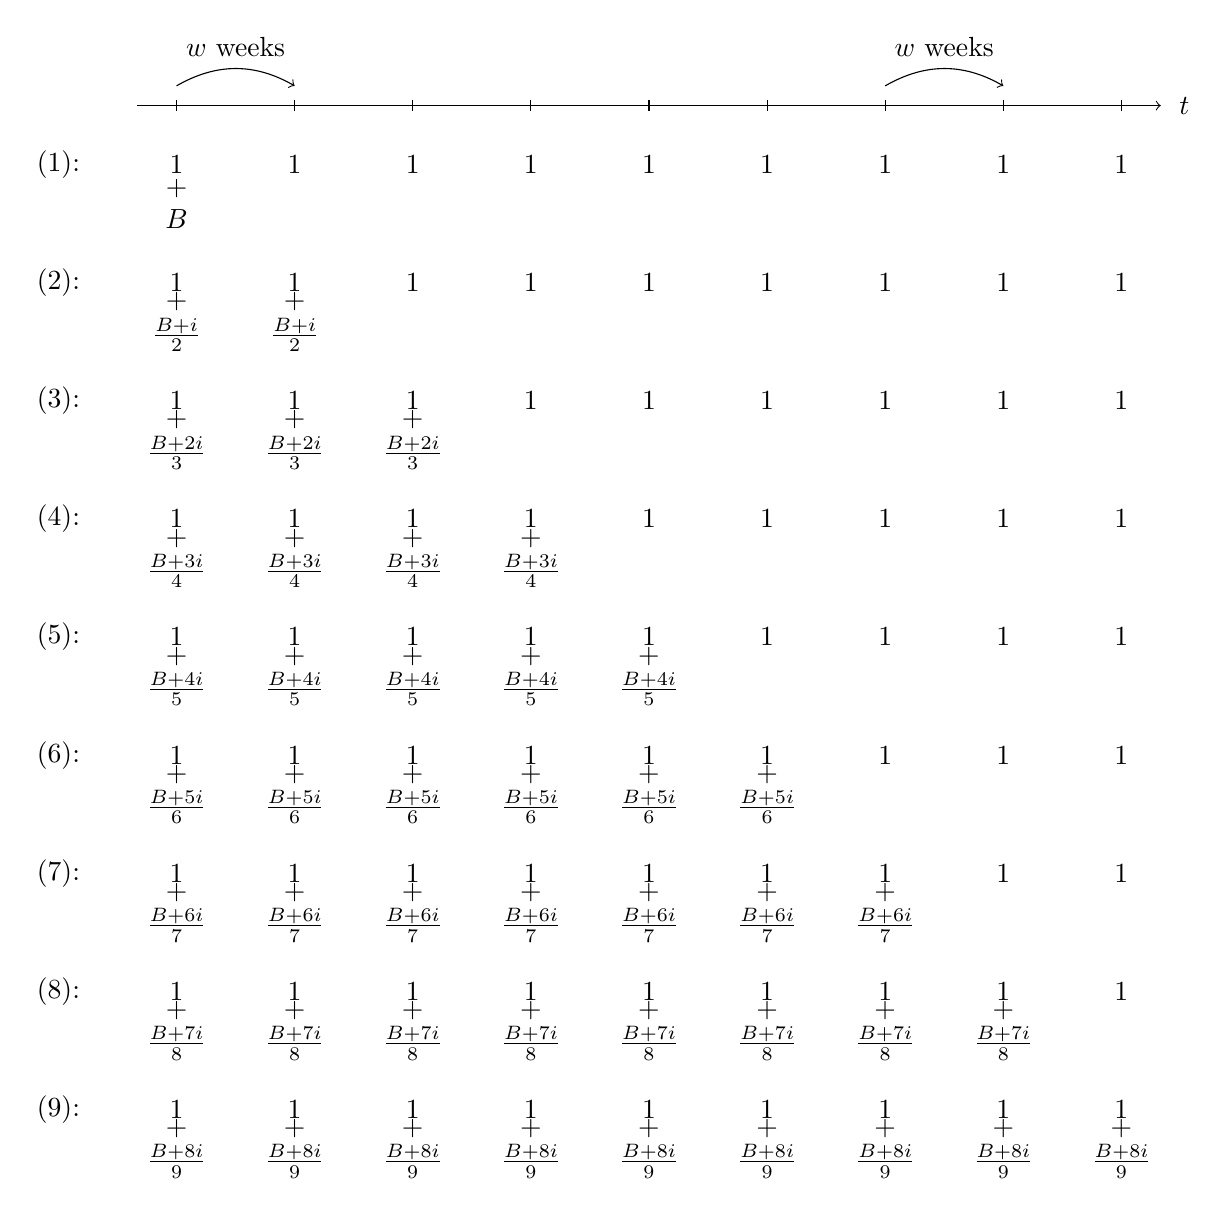
\begin{tikzpicture}
		
		\draw[->] (-9.5,0) -- (3.5,0); 
		\node at (3.8,0) {$t$};
		\node at (-8.25,0.75) {$w$ weeks};
		\path[->] (-9,0.25) edge [bend left] (-7.5,0.25);
		\node at (0.75,0.75) {$w$ weeks};
		\path[->] (0,0.25) edge [bend left] (1.5,0.25);
		%\node at (-10,0.2) {(i):}; % 1
		
		\draw (-9,0.075) -- (-9,-0.075); %node at (-9,0.3) {$1$};
		\draw (-7.5,0.075) -- (-7.5,-0.075); %node at (-7.5,0.3) {$2$};
		\draw (-6,0.075) -- (-6,-0.075); %node at (-6,0.3) {$3$};
		\draw (-4.5,0.075) -- (-4.5,-0.075); %node at (-4.5,0.3) {$4$};
		\draw (-3,0.075) -- (-3,-0.075); %node at (-3,0.3) {$5$};
		\draw (-1.5,0.075) -- (-1.5,-0.075); %node at (-1.5,0.3) {$6$};
		\draw (0,0.075) -- (0,-0.075); %node at (0,0.3) {$7$};
		\draw (1.5,0.075) -- (1.5,-0.075); %node at (1.5,0.3) {$8$};
		\draw (3,0.075) -- (3,-0.075); %node at (3,0.3) {$9$};
		
		
		\node at (-10.5,-.75) {$\cunbalCLA(1)$:};
		\node at (-9,-.75) {$1$};
		\node[align = center] at (-9,-1.25) {$+$ \\ $B$};
		\node at (-7.5,-.75) {$1$};
		\node at (-6,-.75) {$1$};
		\node at (-4.5,-.75) {$1$};
		\node at (-3,-.75) {$1$};
		\node at (-1.5,-.75) {$1$};
		\node at (0,-.75) {$1$};
		\node at (1.5,-.75) {$1$};
		\node at (3,-.75) {$1$};
		
		\node at (-10.5,-2.25) {$\cunbalCLA(2)$:}; 
		
		\node at (-9,-2.25) {$1$};
		\node[align = center] at (-9,-2.75) {$+$ \\ $\frac{B+i}{2}$};
		\node[align = center] at (-7.5,-2.75) {$+$ \\ $\frac{B+i}{2}$};
		\node at (-7.5,-2.25) {$1$};
		\node at (-6,-2.25) {$1$};
		\node at (-4.5,-2.25) {$1$};
		\node at (-3,-2.25) {$1$};
		\node at (-1.5,-2.25) {$1$};
		\node at (0,-2.25) {$1$};
		\node at (1.5,-2.25) {$1$};
		\node at (3,-2.25) {$1$};
		
		\node at (-10.5,-3.75) {$\cunbalCLA(3)$:}; 
		\node[align = center] at (-9,-4.25) {$+$ \\ $\frac{B+2i}{3}$};
		\node[align = center] at (-7.5,-4.25) {$+$ \\ $\frac{B+2i}{3}$};
		\node[align = center] at (-6,-4.25) {$+$ \\ $\frac{B+2i}{3}$};
		\node at (-9,-3.75) {$1$};
		\node at (-7.5,-3.75) {$1$};
		\node at (-6,-3.75) {$1$};
		\node at (-4.5,-3.75) {$1$};
		\node at (-3,-3.75) {$1$};
		\node at (-1.5,-3.75) {$1$};
		\node at (0,-3.75) {$1$};
		\node at (1.5,-3.75) {$1$};
		\node at (3,-3.75) {$1$};
		
		\node at (-10.5,-5.25) {$\cunbalCLA(4)$:}; 
		\node[align = center] at (-9,-5.75) {$+$ \\ $\frac{B+3i}{4}$};
		\node[align = center] at (-7.5,-5.75) {$+$ \\ $\frac{B+3i}{4}$};
		\node[align = center] at (-6,-5.75) {$+$ \\ $\frac{B+3i}{4}$};
		\node[align = center] at (-4.5,-5.75) {$+$ \\ $\frac{B+3i}{4}$};
		\node at (-9,-5.25) {$1$};
		\node at (-7.5,-5.25) {$1$};
		\node at (-6,-5.25) {$1$};
		\node at (-4.5,-5.25) {$1$};
		\node at (-3,-5.25) {$1$};
		\node at (-1.5,-5.25) {$1$};
		\node at (0,-5.25) {$1$};
		\node at (1.5,-5.25) {$1$};
		\node at (3,-5.25) {$1$};
		
		\node at (-10.5,-6.75) {$\cunbalCLA(5)$:}; 
		\node[align = center] at (-9,-7.25) {$+$ \\ $\frac{B+4i}{5}$};
		\node[align = center] at (-7.5,-7.25) {$+$ \\ $\frac{B+4i}{5}$};
		\node[align = center] at (-6,-7.25) {$+$ \\ $\frac{B+4i}{5}$};
		\node[align = center] at (-4.5,-7.25) {$+$ \\ $\frac{B+4i}{5}$};
		\node[align = center] at (-3,-7.25) {$+$ \\ $\frac{B+4i}{5}$};
		\node at (-9,-6.75) {$1$};
		\node at (-7.5,-6.75) {$1$};
		\node at (-6,-6.75) {$1$};
		\node at (-4.5,-6.75) {$1$};
		\node at (-3,-6.75) {$1$};
		\node at (-1.5,-6.75) {$1$};
		\node at (0,-6.75) {$1$};
		\node at (1.5,-6.75) {$1$};
		\node at (3,-6.75) {$1$};
		
		\node at (-10.5,-8.25) {$\cunbalCLA(6)$:}; 
		\node[align = center] at (-9,-8.75) {$+$ \\ $\frac{B+5i}{6}$};
		\node[align = center] at (-7.5,-8.75) {$+$ \\ $\frac{B+5i}{6}$};
		\node[align = center] at (-6,-8.75) {$+$ \\ $\frac{B+5i}{6}$};
		\node[align = center] at (-4.5,-8.75) {$+$ \\ $\frac{B+5i}{6}$};
		\node[align = center] at (-3,-8.75) {$+$ \\ $\frac{B+5i}{6}$};
		\node[align = center] at (-1.5,-8.75) {$+$ \\ $\frac{B+5i}{6}$};
		\node at (-9,-8.25) {$1$};
		\node at (-7.5,-8.25) {$1$};
		\node at (-6,-8.25) {$1$};
		\node at (-4.5,-8.25) {$1$};
		\node at (-3,-8.25) {$1$};
		\node at (-1.5,-8.25) {$1$};
		\node at (0,-8.25) {$1$};
		\node at (1.5,-8.25) {$1$};
		\node at (3,-8.25) {$1$};
		
		\node at (-10.5,-9.75) {$\cunbalCLA(7)$:};
		\node[align = center] at (-9,-10.25) {$+$ \\ $\frac{B+6i}{7}$};
		\node[align = center] at (-7.5,-10.25) {$+$ \\ $\frac{B+6i}{7}$};
		\node[align = center] at (-6,-10.25) {$+$ \\ $\frac{B+6i}{7}$};
		\node[align = center] at (-4.5,-10.25) {$+$ \\ $\frac{B+6i}{7}$};
		\node[align = center] at (-3,-10.25) {$+$ \\ $\frac{B+6i}{7}$};
		\node[align = center] at (-1.5,-10.25) {$+$ \\ $\frac{B+6i}{7}$};
		\node[align = center] at (0,-10.25) {$+$ \\ $\frac{B+6i}{7}$}; 
		\node at (-9,-9.75) {$1$};
		\node at (-7.5,-9.75) {$1$};
		\node at (-6,-9.75) {$1$};
		\node at (-4.5,-9.75) {$1$};
		\node at (-3,-9.75) {$1$};
		\node at (-1.5,-9.75) {$1$};
		\node at (0,-9.75) {$1$};
		\node at (1.5,-9.75) {$1$};
		\node at (3,-9.75) {$1$};
		
		\node at (-10.5,-11.25) {$\cunbalCLA(8)$:};
		\node[align = center] at (-9,-11.75) {$+$ \\ $\frac{B+7i}{8}$};
		\node[align = center] at (-7.5,-11.75) {$+$ \\ $\frac{B+7i}{8}$};
		\node[align = center] at (-6,-11.75) {$+$ \\ $\frac{B+7i}{8}$};
		\node[align = center] at (-4.5,-11.75) {$+$ \\ $\frac{B+7i}{8}$};
		\node[align = center] at (-3,-11.75) {$+$ \\ $\frac{B+7i}{8}$};
		\node[align = center] at (-1.5,-11.75) {$+$ \\ $\frac{B+7i}{8}$};
		\node[align = center] at (0,-11.75) {$+$ \\ $\frac{B+7i}{8}$};
		\node[align = center] at (1.5,-11.75) {$+$ \\ $\frac{B+7i}{8}$};
		\node at (-9,-11.25) {$1$};
		\node at (-7.5,-11.25) {$1$};
		\node at (-6,-11.25) {$1$};
		\node at (-4.5,-11.25) {$1$};
		\node at (-3,-11.25) {$1$};
		\node at (-1.5,-11.25) {$1$};
		\node at (0,-11.25) {$1$};
		\node at (1.5,-11.25) {$1$};
		\node at (3,-11.25) {$1$};
		
		\node at (-10.5,-12.75) {$\cunbalCLA(9)$:}; 
		\node[align = center] at (-9,-13.25) {$+$ \\ $\frac{B+8i}{9}$};
		\node[align = center] at (-7.5,-13.25) {$+$ \\ $\frac{B+8i}{9}$};
		\node[align = center] at (-6,-13.25) {$+$ \\ $\frac{B+8i}{9}$};
		\node[align = center] at (-4.5,-13.25) {$+$ \\ $\frac{B+8i}{9}$};
		\node[align = center] at (-3,-13.25) {$+$ \\ $\frac{B+8i}{9}$};
		\node[align = center] at (-1.5,-13.25) {$+$ \\ $\frac{B+8i}{9}$};
		\node[align = center] at (0,-13.25) {$+$ \\ $\frac{B+8i}{9}$};
		\node[align = center] at (1.5,-13.25){$+$ \\ $\frac{B+8i}{9}$};
		\node[align = center] at (3,-13.25) {$+$ \\ $\frac{B+8i}{9}$};
		\node at (-9,-12.75) {$1$};
		\node at (-7.5,-12.75) {$1$};
		\node at (-6,-12.75) {$1$};
		\node at (-4.5,-12.75) {$1$};
		\node at (-3,-12.75) {$1$};
		\node at (-1.5,-12.75) {$1$};
		\node at (0,-12.75) {$1$};
		\node at (1.5,-12.75) {$1$};
		\node at (3,-12.75) {$1$};
		
		\end{tikzpicture}
	}
	\caption{Earnings Sequences Included in Choice List $\CunbalCLA$}
	\label{fig:incrdisp_cl}
	\tablenotes[Notes:]{%
		For the values of $B$, $i$, and $w$ that we used see \autoref{sec:Methods}.
		Figure taken from \cite{Dertwinkel-Kalt2017}.
	}
\end{figure}

\begin{figure}[h]
	\resizebox{\textwidth}{!}{
		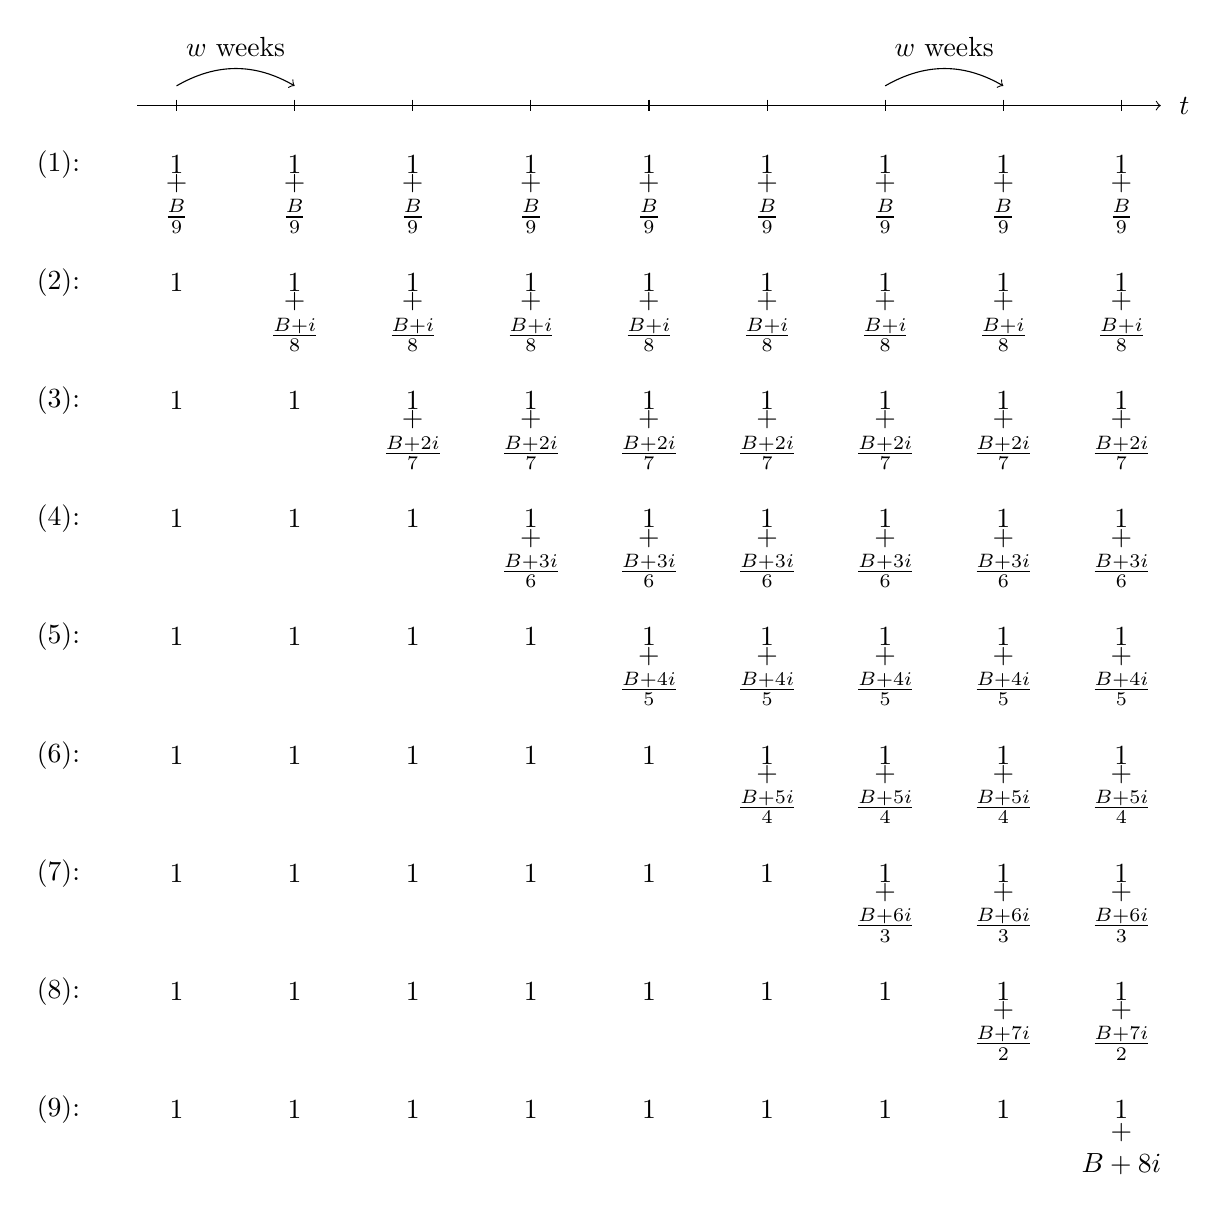
\begin{tikzpicture}
		
		
		\draw[->] (-9.5,0) -- (3.5,0); 
		\node at (3.8,0) {$t$};
		\node at (-8.25,0.75) {$w$ weeks};
		\path[->] (-9,0.25) edge [bend left] (-7.5,0.25);
		\node at (0.75,0.75) {$w$ weeks};
		\path[->] (0,0.25) edge [bend left] (1.5,0.25);
		%\node at (-10,0.2) {(i):}; % 1
		
		\draw (-9,0.075) -- (-9,-0.075); %node at (-9,0.3) {$1$};
		\draw (-7.5,0.075) -- (-7.5,-0.075); %node at (-7.5,0.3) {$2$};
		\draw (-6,0.075) -- (-6,-0.075); %node at (-6,0.3) {$3$};
		\draw (-4.5,0.075) -- (-4.5,-0.075); %node at (-4.5,0.3) {$4$};
		\draw (-3,0.075) -- (-3,-0.075); %node at (-3,0.3) {$5$};
		\draw (-1.5,0.075) -- (-1.5,-0.075); %node at (-1.5,0.3) {$6$};
		\draw (0,0.075) -- (0,-0.075); %node at (0,0.3) {$7$};
		\draw (1.5,0.075) -- (1.5,-0.075); %node at (1.5,0.3) {$8$};
		\draw (3,0.075) -- (3,-0.075); %node at (3,0.3) {$9$};
		
		
		\node at (-10.5,-.75) {$\cunbalCLB(1)$:}; 
		
		\node at (-9,-.75) {$1$};
		\node[align = center] at (-9,-1.25) {$+$ \\ $\frac{B}{9}$};
		\node at (-7.5,-.75) {$1$};
		\node[align = center] at (-7.5,-1.25) {$+$ \\ $\frac{B}{9}$};
		\node at (-6,-.75) {$1$};
		\node[align = center] at (-6,-1.25) {$+$ \\ $\frac{B}{9}$};
		\node at (-4.5,-.75) {$1$};
		\node[align = center] at (-4.5,-1.25) {$+$ \\ $\frac{B}{9}$};
		\node at (-3,-.75) {$1$};
		\node[align = center] at (-3,-1.25) {$+$ \\ $\frac{B}{9}$};
		\node at (-1.5,-.75) {$1$};
		\node[align = center] at (-1.5,-1.25) {$+$ \\ $\frac{B}{9}$};
		\node at (0,-.75) {$1$};
		\node[align = center] at (0,-1.25) {$+$ \\ $\frac{B}{9}$};
		\node at (1.5,-.75) {$1$};
		\node[align = center] at (1.5,-1.25) {$+$ \\ $\frac{B}{9}$};
		\node at (3,-.75) {$1$};
		\node[align = center] at (3,-1.25) {$+$ \\ $\frac{B}{9}$};
		
		\node at (-10.5,-2.25) {$\cunbalCLB(2)$:};
		\node at (-9,-2.25) {$1$};
		\node at (-7.5,-2.25) {$1$};
		\node[align = center] at (-7.5,-2.75) {$+$ \\ $\frac{B+i}{8}$};
		\node at (-6,-2.25) {$1$};
		\node[align = center] at (-6,-2.75) {$+$ \\ $\frac{B+i}{8}$};
		\node at (-4.5,-2.25) {$1$};
		\node[align = center] at (-4.5,-2.75) {$+$ \\ $\frac{B+i}{8}$};
		\node at (-3,-2.25) {$1$};
		\node[align = center] at (-3,-2.75) {$+$ \\ $\frac{B+i}{8}$};
		\node at (-1.5,-2.25) {$1$};
		\node[align = center] at (-1.5,-2.75) {$+$ \\ $\frac{B+i}{8}$};
		\node at (0,-2.25) {$1$};
		\node[align = center] at (0,-2.75) {$+$ \\ $\frac{B+i}{8}$};
		\node at (1.5,-2.25) {$1$};
		\node[align = center] at (1.5,-2.75) {$+$ \\ $\frac{B+i}{8}$};
		\node at (3,-2.25) {$1$};
		\node[align = center] at (3,-2.75) {$+$ \\ $\frac{B+i}{8}$};
		
		\node at (-10.5,-3.75) {$\cunbalCLB(3)$:}; 
		\node at (-9,-3.75) {$1$};
		\node at (-7.5,-3.75) {$1$};
		\node at (-6,-3.75) {$1$};
		\node[align = center] at (-6,-4.25) {$+$ \\ $\frac{B+2i}{7}$};
		\node at (-4.5,-3.75) {$1$};
		\node[align = center] at (-4.5,-4.25) {$+$ \\ $\frac{B+2i}{7}$};
		\node at (-3,-3.75) {$1$};
		\node[align = center] at (-3,-4.25) {$+$ \\ $\frac{B+2i}{7}$};
		\node at (-1.5,-3.75) {$1$};
		\node[align = center] at (-1.5,-4.25) {$+$ \\ $\frac{B+2i}{7}$};
		\node at (0,-3.75) {$1$};
		\node[align = center] at (0,-4.25) {$+$ \\ $\frac{B+2i}{7}$};
		\node at (1.5,-3.75) {$1$};
		\node[align = center] at (1.5,-4.25) {$+$ \\ $\frac{B+2i}{7}$};
		\node at (3,-3.75) {$1$};
		\node[align = center] at (3,-4.25) {$+$ \\ $\frac{B+2i}{7}$};
		
		\node at (-10.5,-5.25) {$\cunbalCLB(4)$:}; 
		\node at (-9,-5.25) {$1$};
		\node at (-7.5,-5.25) {$1$};
		\node at (-6,-5.25) {$1$};
		\node at (-4.5,-5.25) {$1$};
		\node[align = center] at (-4.5,-5.75) {$+$ \\ $\frac{B+3i}{6}$};
		\node at (-3,-5.25) {$1$};
		\node[align = center] at (-3,-5.75) {$+$ \\ $\frac{B+3i}{6}$};
		\node at (-1.5,-5.25) {$1$};
		\node[align = center] at (-1.5,-5.75) {$+$ \\ $\frac{B+3i}{6}$};
		\node at (0,-5.25) {$1$};
		\node[align = center] at (0,-5.75) {$+$ \\ $\frac{B+3i}{6}$};
		\node at (1.5,-5.25) {$1$};
		\node[align = center] at (1.5,-5.75) {$+$ \\ $\frac{B+3i}{6}$};
		\node at (3,-5.25) {$1$};
		\node[align = center] at (3,-5.75) {$+$ \\ $\frac{B+3i}{6}$};
		
		\node at (-10.5,-6.75) {$\cunbalCLB(5)$:}; 
		\node at (-9,-6.75) {$1$};
		\node at (-7.5,-6.75) {$1$};
		\node at (-6,-6.75) {$1$};
		\node at (-4.5,-6.75) {$1$};
		\node at (-3,-6.75) {$1$};
		\node[align = center] at (-3,-7.25) {$+$ \\ $\frac{B+4i}{5}$};
		\node at (-1.5,-6.75) {$1$};
		\node[align = center] at (-1.5,-7.25) {$+$ \\ $\frac{B+4i}{5}$};
		\node at (0,-6.75) {$1$};
		\node[align = center] at (0,-7.25) {$+$ \\ $\frac{B+4i}{5}$};
		\node at (1.5,-6.75) {$1$};
		\node[align = center] at (1.5,-7.25) {$+$ \\ $\frac{B+4i}{5}$};
		\node at (3,-6.75) {$1$};
		\node[align = center] at (3,-7.25) {$+$ \\ $\frac{B+4i}{5}$};
		
		\node at (-10.5,-8.25) {$\cunbalCLB(6)$:}; 
		\node at (-9,-8.25) {$1$};
		\node at (-7.5,-8.25) {$1$};
		\node at (-6,-8.25) {$1$};
		\node at (-4.5,-8.25) {$1$};
		\node at (-3,-8.25) {$1$};
		\node at (-1.5,-8.25) {$1$};
		\node[align = center] at (-1.5,-8.75) {$+$ \\ $\frac{B+5i}{4}$};
		\node at (0,-8.25) {$1$};
		\node[align = center] at (0,-8.75) {$+$ \\ $\frac{B+5i}{4}$};
		\node at (1.5,-8.25) {$1$};
		\node[align = center] at (1.5,-8.75) {$+$ \\ $\frac{B+5i}{4}$};
		\node at (3,-8.25) {$1$};
		\node[align = center] at (3,-8.75) {$+$ \\ $\frac{B+5i}{4}$};
		
		\node at (-10.5,-9.75) {$\cunbalCLB(7)$:}; 
		\node at (-9,-9.75) {$1$};
		\node at (-7.5,-9.75) {$1$};
		\node at (-6,-9.75) {$1$};
		\node at (-4.5,-9.75) {$1$};
		\node at (-3,-9.75) {$1$};
		\node at (-1.5,-9.75) {$1$};
		\node at (0,-9.75) {$1$};
		\node[align = center] at (0,-10.25) {$+$ \\ $\frac{B+6i}{3}$};
		\node at (1.5,-9.75) {$1$};
		\node[align = center] at (1.5,-10.25) {$+$ \\ $\frac{B+6i}{3}$};
		\node at (3,-9.75) {$1$};
		\node[align = center] at (3,-10.25) {$+$ \\ $\frac{B+6i}{3}$};
		
		\node at (-10.5,-11.25) {$\cunbalCLB(8)$:}; 
		\node at (-9,-11.25) {$1$};
		\node at (-7.5,-11.25) {$1$};
		\node at (-6,-11.25) {$1$};
		\node at (-4.5,-11.25) {$1$};
		\node at (-3,-11.25) {$1$};
		\node at (-1.5,-11.25) {$1$};
		\node at (0,-11.25) {$1$};
		\node at (1.5,-11.25) {$1$};
		\node[align = center] at (1.5,-11.75) {$+$ \\ $\frac{B+7i}{2}$};
		\node at (3,-11.25) {$1$};
		\node[align = center] at (3,-11.75) {$+$ \\ $\frac{B+7i}{2}$};
		
		\node at (-10.5,-12.75) {$\cunbalCLB(9)$:}; 
		\node[align = center] at (3,-13.25){$+$ \\ $B + 8i$};
		\node at (-9,-12.75) {$1$};
		\node at (-7.5,-12.75) {$1$};
		\node at (-6,-12.75) {$1$};
		\node at (-4.5,-12.75) {$1$};
		\node at (-3,-12.75) {$1$};
		\node at (-1.5,-12.75) {$1$};
		\node at (0,-12.75) {$1$};
		\node at (1.5,-12.75) {$1$};
		\node at (3,-12.75) {$1$};
		
		\end{tikzpicture}
	}
	\caption{Earnings Sequences Included in Choice List $\CunbalCLB$}
	\label{fig:decrdisp_cl}
	\tablenotes[Notes:]{%
		For the values of $B$, $i$, and $w$ that we used see \autoref{sec:Methods}.
		Figure taken from \cite{Dertwinkel-Kalt2017}.
	}
\end{figure}